\documentclass{standalone}
\usepackage{graphicx}	
\usepackage{amssymb, amsmath, amsthm}
\usepackage{color}

\usepackage{tikz}
\usetikzlibrary{intersections, backgrounds}

\definecolor{light}{RGB}{220, 188, 188}
\definecolor{mid}{RGB}{185, 124, 124}
\definecolor{dark}{RGB}{143, 39, 39}
\definecolor{highlight}{RGB}{180, 31, 180}
\definecolor{gray10}{gray}{0.1}
\definecolor{gray20}{gray}{0.2}
\definecolor{gray30}{gray}{0.3}
\definecolor{gray40}{gray}{0.4}
\definecolor{gray60}{gray}{0.6}
\definecolor{gray70}{gray}{0.7}
\definecolor{gray80}{gray}{0.8}
\definecolor{gray90}{gray}{0.9}
\definecolor{gray95}{gray}{0.95}

\begin{document}

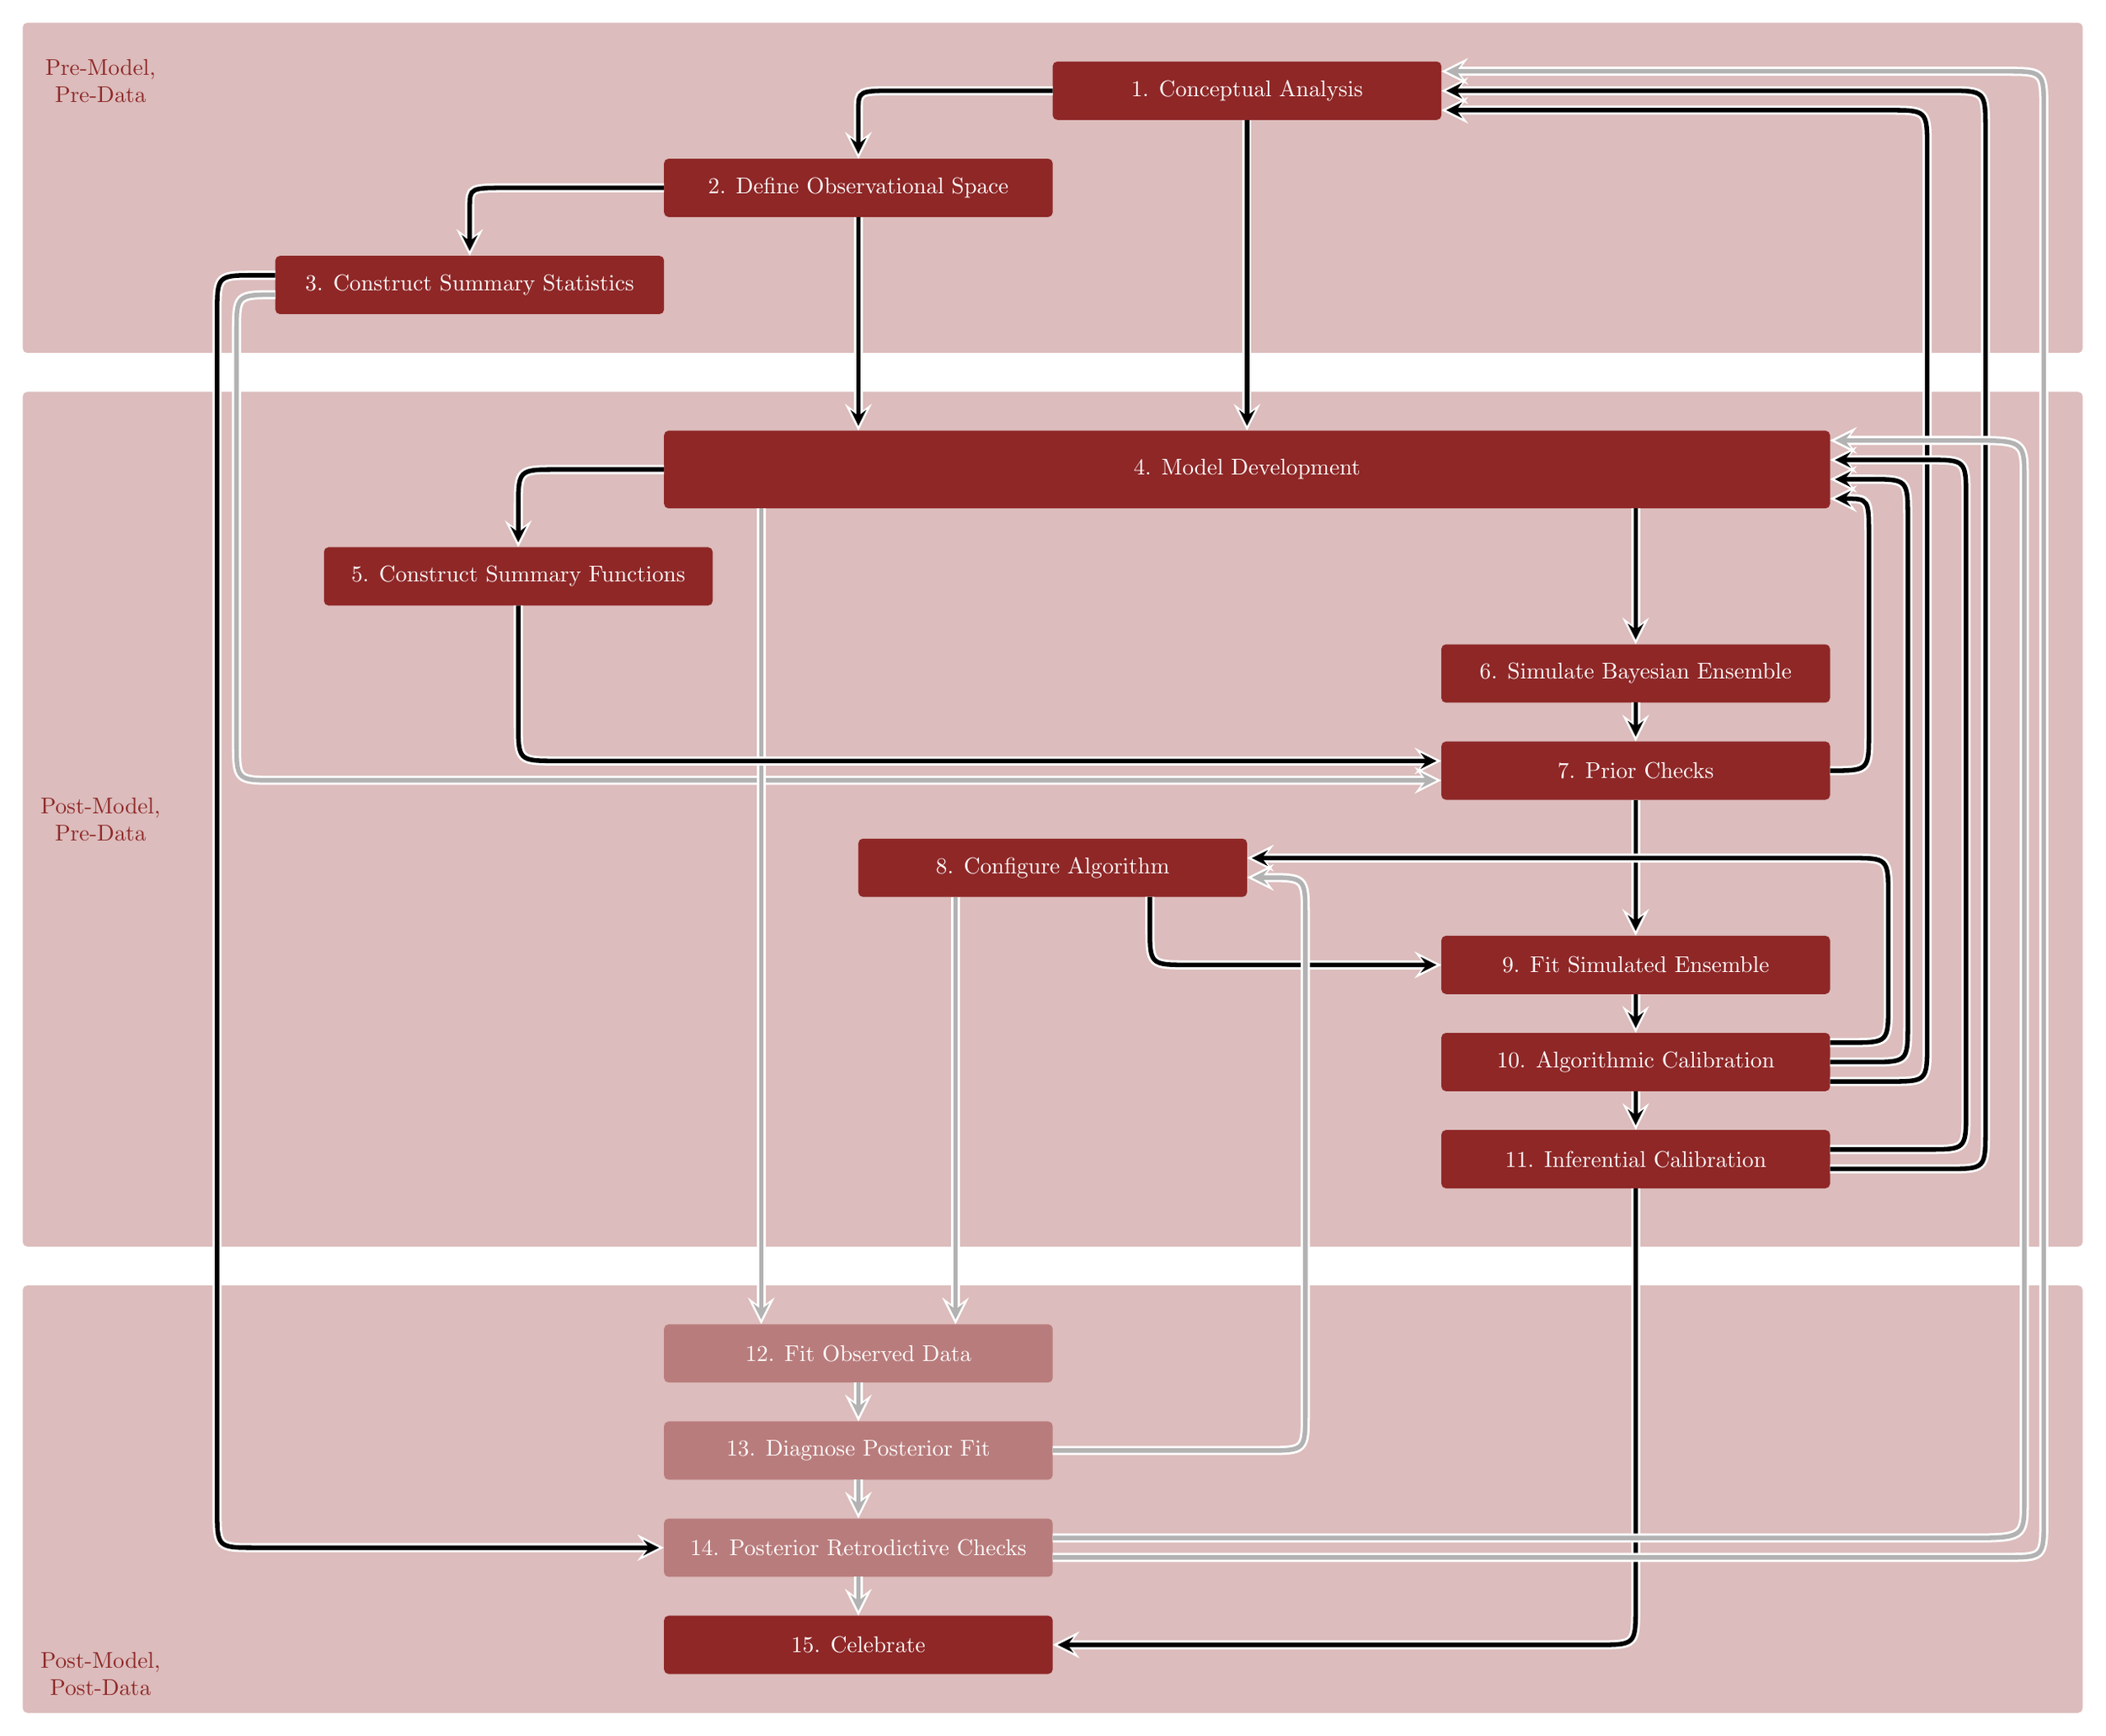
\begin{tikzpicture}[scale=0.3, thick]

  % Pre Model, Pre Data
  \fill [rounded corners=2pt, light] (-73, 63) rectangle (33, 80);
  \node[align=center, dark] at (-69, 77) { Pre-Model,\\Pre-Data};
  
  % Post Model, Pre Data
  \fill [rounded corners=2pt, light] (-73, 17) rectangle (33, 61);
  \node[align=center, dark] at (-69, 39) { Post-Model,\\Pre-Data};
 
  % Post Model, Post Data
  \fill [rounded corners=2pt, light] (-73, -7) rectangle (33, 15);
  \node[align=center, dark] at (-69, -5) { Post-Model,\\Post-Data};
  
  % Step One
  \fill [rounded corners=2pt, fill=dark, text=white] (-20, 75) rectangle +(20, 3) 
  node [midway, align=center] {1. Conceptual Analysis};

  \draw [->, >=stealth, white, line width=4] (-10, 75) -- (-10, 59);
  \draw [->, >=stealth, line width=2] (-10, 75) -- (-10, 59.25);
  
  \draw [->, >=stealth, white, line width=4] 
    (-20, 76.5) -- (-28, 76.5) .. controls (-30, 76.5) .. (-30, 75.5) -- (-30, 73);
  \draw [->, >=stealth, line width=2] 
    (-20, 76.5) -- (-28, 76.5) .. controls (-30, 76.5) .. (-30, 75.5) -- (-30, 73.25);

  % Step Two
  \fill [rounded corners=2pt, fill=dark, text=white] (-40, 70) rectangle +(20, 3) 
  node [midway, align=center] {2. Define Observational Space};

  \draw [->, >=stealth, white, line width=4] (-30, 70) -- (-30, 59);
  \draw [->, >=stealth, line width=2] (-30, 70) -- (-30, 59.25);

  \draw [->, >=stealth, white, line width=4] 
    (-40, 71.5) -- (-48, 71.5) .. controls (-50, 71.5) .. (-50, 70.5) -- (-50, 68);
  \draw [->, >=stealth, line width=2] 
    (-40, 71.5) -- (-48, 71.5) .. controls (-50, 71.5) .. (-50, 70.5) -- (-50, 68.25);
  
  % Step Three
  \fill [rounded corners=2pt, fill=dark, text=white] (-60, 65) rectangle +(20, 3) 
  node [midway, align=center] {3. Construct Summary Statistics};

  \draw [->, >=stealth, white, line width=4] 
    (-60, 66) .. controls (-62, 66) .. (-62, 64) --
    (-62, 43) .. controls (-62, 41) .. (-60, 41) -- (0, 41);
  
  \draw [->, >=stealth, gray70, line width=2] 
    (-60, 66) .. controls (-62, 66) .. (-62, 64) --
    (-62, 43) .. controls (-62, 41) .. (-60, 41) -- (-0.25, 41);

  \draw [->, >=stealth, white, line width=4] 
    (-60, 67) -- (-61, 67) .. controls (-63, 67) .. (-63, 65) --
    (-63, 3.5) .. controls (-63, 1.5) .. (-61, 1.5) -- (-40, 1.5);

  \draw [->, >=stealth, line width=2] 
    (-60, 67) -- (-61, 67) .. controls (-63, 67) .. (-63, 65) --
    (-63, 3.5) .. controls (-63, 1.5) .. (-61, 1.5) -- (-40.25, 1.5);

  % Step Four
  \fill [rounded corners=2pt, fill=dark, text=white] (-40, 55) rectangle +(60, 4) 
  node [midway, align=center] {4. Model Development};
  
  \draw [->, >=stealth, white, line width=4] (10, 55) -- (10, 48);
  \draw [->, >=stealth, line width=2] (10, 55) -- (10, 48.25);

  \draw [->, >=stealth, white, line width=4] (-35, 55) -- (-35, 13);
  \draw [->, >=stealth, gray70, line width=2] (-35, 55) -- (-35, 13.25);

  \draw [->, >=stealth, white, line width=4] 
    (-40, 57) -- (-45.5, 57) .. controls (-47.5, 57) .. (-47.5, 55) -- (-47.5, 53);
  \draw [->, >=stealth, line width=2] 
    (-40, 57) -- (-45.5, 57) .. controls (-47.5, 57) .. (-47.5, 55) -- (-47.5, 53.25);
  
  % Step Five
  \fill [rounded corners=2pt, fill=dark, text=white] (-57.5, 50) rectangle +(20, 3) 
  node [midway, align=center] {5. Construct Summary Functions};
  
  \draw [->, >=stealth, white, line width=4] 
    (-47.5, 50) -- (-47.5, 44) .. controls (-47.5, 42) .. (-45.5, 42) -- (0, 42);  
  \draw [->, >=stealth, line width=2] 
    (-47.5, 50) -- (-47.5, 44) .. controls (-47.5, 42) .. (-45.5, 42) -- (-0.25, 42);  
       
  % Step Six
  \fill [rounded corners=2pt, fill=dark, text=white] (0, 45) rectangle +(20, 3) 
  node [midway, align=center] {6. Simulate Bayesian Ensemble};
  
  \draw [->, >=stealth, white, line width=4] (10, 45) -- (10, 43);
  \draw [->, >=stealth, line width=2] (10, 45) -- (10, 43.25);
  
  % Step Seven
  \fill [rounded corners=2pt, fill=dark, text=white] (0, 40) rectangle +(20, 3) 
  node [midway, align=center] {7. Prior Checks};
  
  \draw [->, >=stealth, white, line width=4] (10, 40) -- (10, 33);
  \draw [->, >=stealth, line width=2] (10, 40) -- (10, 33.25);

  \draw [->, >=stealth, white, line width=4] 
    (20, 41.5) .. controls (22, 41.5) .. (22, 43.5) -- 
    (22, 53.5) .. controls (22, 55.5) .. (20, 55.5);
  
  \draw [->, >=stealth, line width=2] 
    (20, 41.5) .. controls (22, 41.5) .. (22, 43.5) -- 
    (22, 53.5) .. controls (22, 55.5) .. (20 + 0.25, 55.5);
  
  % Step Eight
  \fill [rounded corners=2pt, fill=dark, text=white] (-30, 35) rectangle +(20, 3) 
  node [midway, align=center] {8. Configure Algorithm};
  
  \draw [->, >=stealth, white, line width=4] (-25, 35) -- (-25, 13);
  \draw [->, >=stealth, gray70, line width=2] (-25, 35) -- (-25, 13.25);
  
  \draw [->, >=stealth, white, line width=4] 
    (-15, 35) -- (-15, 33.5) .. controls (-15, 31.5) .. (-13, 31.5) -- (0, 31.5);  
  \draw [->, >=stealth, line width=2] 
    (-15, 35) -- (-15, 33.5) .. controls (-15, 31.5) .. (-13, 31.5) -- (-0.25, 31.5);
  
  % Step Nine
  \fill [rounded corners=2pt, fill=dark, text=white] (0, 30) rectangle +(20, 3) 
  node [midway, align=center] {9. Fit Simulated Ensemble};
  
  \draw [->, >=stealth, white, line width=4] (10, 30) -- (10, 28);
  \draw [->, >=stealth, line width=2] (10, 30) -- (10, 28.25);
  
  % Step Ten
  \fill [rounded corners=2pt, fill=dark, text=white] (0, 25) rectangle +(20, 3) 
  node [midway, align=center] {10. Algorithmic Calibration};
  
  \draw [->, >=stealth, white, line width=4] (10, 25) -- (10, 23);
  \draw [->, >=stealth, line width=2] (10, 25) -- (10, 23.25);

  \draw [->, >=stealth, white, line width=4] 
    (20, 27.5) -- (21, 27.5) .. controls (23, 27.5) .. (23, 29.5) -- 
    (23, 35) .. controls (23, 37) .. (21, 37) -- (-10, 37);
  
  \draw [->, >=stealth, line width=2] 
    (20, 27.5) -- (21, 27.5) .. controls (23, 27.5) .. (23, 29.5) -- 
    (23, 35) .. controls (23, 37) .. (21, 37) -- (-10 + 0.25, 37);

  \draw [->, >=stealth, white, line width=4] 
    (20, 26.5) -- (22, 26.5) .. controls (24, 26.5) .. (24, 28.5) -- 
    (24, 54.5) .. controls (24, 56.5) .. (22, 56.5) -- (20, 56.5);

  \draw [->, >=stealth, line width=2] 
    (20, 26.5) -- (22, 26.5) .. controls (24, 26.5) .. (24, 28.5) -- 
    (24, 54.5) .. controls (24, 56.5) .. (22, 56.5) -- (20 + 0.25, 56.5);

  \draw [->, >=stealth, white, line width=4] 
    (20, 25.5) -- (23, 25.5) .. controls (25, 25.5) .. (25, 27.5) -- 
    (25, 73.5) .. controls (25, 75.5) .. (23, 75.5) -- (0, 75.5);

  \draw [->, >=stealth, line width=2] 
    (20, 25.5) -- (23, 25.5) .. controls (25, 25.5) .. (25, 27.5) -- 
    (25, 73.5) .. controls (25, 75.5) .. (23, 75.5) -- (0.25, 75.5);
  
  % Step Eleven
  \fill [rounded corners=2pt, fill=dark, text=white] (0, 20) rectangle +(20, 3) 
  node [midway, align=center] {11. Inferential Calibration};

  \draw [->, >=stealth, white, line width=4] 
    (20, 22) -- (25, 22) .. controls (27, 22) .. (27, 24) -- 
    (27, 55.5) .. controls (27, 57.5) .. (25, 57.5) -- (20, 57.5);

  \draw [->, >=stealth, line width=2] 
    (20, 22) -- (25, 22) .. controls (27, 22) .. (27, 24) -- 
    (27, 55.5) .. controls (27, 57.5) .. (25, 57.5) -- (20 + 0.25, 57.5);

  \draw [->, >=stealth, white, line width=4] 
    (20, 21) -- (26, 21) .. controls (28, 21) .. (28, 23) --
    (28, 74.5) .. controls (28, 76.5) .. (26, 76.5) -- (0, 76.5); 
  
  \draw [->, >=stealth, line width=2] 
    (20, 21) -- (26, 21) .. controls (28, 21) .. (28, 23) --
    (28, 74.5) .. controls (28, 76.5) .. (26, 76.5) -- (0.25, 76.5); 
  
  \draw [->, >=stealth, white, line width=4] 
    (10, 20) -- (10, -1.5) .. controls (10, -3.5) .. (8, -3.5) -- (-20, -3.5); 
    
  \draw [->, >=stealth, line width=2] 
    (10, 20) -- (10, -1.5) .. controls (10, -3.5) .. (8, -3.5) -- (-20 + 0.25, -3.5); 

  % Step Twelve
  \fill [rounded corners=2pt, fill=mid, text=white] (-40, 10) rectangle +(20, 3) 
  node [midway, align=center] {12. Fit Observed Data};
  
  \draw [->, >=stealth, white, line width=4] (-30, 10) -- (-30, 8);
  \draw [->, >=stealth, gray70, line width=2] (-30, 10) -- (-30, 8.25);
  
  % Step Thirteen
  \fill [rounded corners=2pt, fill=mid, text=white] (-40, 5) rectangle +(20, 3) 
  node [midway, align=center] {13. Diagnose Posterior Fit};

  \draw [->, >=stealth, white, line width=4] (-30, 5) -- (-30, 3);
  \draw [->, >=stealth, gray70, line width=2] (-30, 5) -- (-30, 3.25);

  \draw [->, >=stealth, white, line width=4] 
    (-20, 6.5) -- (-9, 6.5) .. controls (-7, 6.5) .. (-7, 8.5) -- 
    (-7, 34) .. controls (-7, 36) .. (-9, 36) -- (-10, 36);
  
  \draw [->, >=stealth, gray70, line width=2] 
    (-20, 6.5) -- (-9, 6.5) .. controls (-7, 6.5) .. (-7, 8.5) -- 
    (-7, 34) .. controls (-7, 36) .. (-9, 36) -- (-10 + 0.25, 36);
  
  % Step Fourteen
  \fill [rounded corners=2pt, fill=mid, text=white] (-40, 0) rectangle +(20, 3) 
  node [midway, align=center] {14. Posterior Retrodictive Checks};

  \draw [->, >=stealth, white, line width=4] (-30, 0) -- (-30, -2);
  \draw [->, >=stealth, gray70, line width=2] (-30, 0) -- (-30, -1.75);

  \draw [->, >=stealth, white, line width=4] 
    (-20, 2) -- (27, 2) .. controls (30, 2) .. (30, 4) -- 
    (30, 56.5) .. controls (30, 58.5) .. (27, 58.5) -- (20, 58.5);
  
  \draw [->, >=stealth, gray70, line width=2] 
    (-20, 2) -- (27, 2) .. controls (30, 2) .. (30, 4) -- 
    (30, 56.5) .. controls (30, 58.5) .. (27, 58.5) -- (20 + 0.25, 58.5);

  \draw [->, >=stealth, white, line width=4] 
    (-20, 1) -- (29, 1) .. controls (31, 1) .. (31, 3) --
    (31, 75.5) .. controls (31, 77.5) .. (29, 77.5) -- (0, 77.5); 
  
  \draw [->, >=stealth, gray70, line width=2] 
    (-20, 1) -- (29, 1) .. controls (31, 1) .. (31, 3) --
    (31, 75.5) .. controls (31, 77.5) .. (29, 77.5) -- (0 + 0.25, 77.5); 

  % Step Fifteen
  \fill [rounded corners=2pt, fill=dark, text=white] (-40, -5) rectangle +(20, 3) 
  node [midway, align=center] {15. Celebrate};
  
\end{tikzpicture}

\end{document}  